\documentclass[11pt]{article}
\usepackage[preprint]{acl}
\usepackage{times,latexsym}
\usepackage[T1]{fontenc}
\usepackage[utf8]{inputenc}
\usepackage{microtype,inconsolata,graphicx,booktabs,amsmath,amssymb,array}
\usepackage{tikz}
\usetikzlibrary{arrows.meta,positioning}
\usepackage{fvextra}
\hypersetup{pdftitle={Beyond Arabic Digits: Probing Large Language Model Logical Reasoning Under Symbol-Set Variation},pdfauthor={Arnav Bharti and Dhruv Kumar}}
\title{Beyond Arabic Digits: Probing Large Language Model\newline Logical Reasoning Under Symbol-Set Variation}
\author{Arnav Bharti \and Dhruv Kumar \\
 Department of Computer Science and Information Systems \\
 Birla Institute of Technology and Science, Pilani \\
 \texttt{f20221585@pilani.bits-pilani.ac.in}}
\newcommand{\gpt}{GPT-OSS}
\newcommand{\qwen}{Qwen}
\begin{document}
\maketitle

\begin{abstract}
Sudoku's constraints are unchanged by a bijective substitution of its value labels. We use this property to study performance under symbol-set variation and assess explanations for representation-sensitive outcomes. From 300 certified unique-solution puzzles, we select 60 across three difficulty tiers and render each in nine alphabets for GPT-OSS 120B and Qwen3.8-27B-FP8. Alphabet accuracy ranges from 61.7\% to 75.0\% for GPT-OSS and from 80.0\% to 93.3\% for Qwen, although no Arabic-baseline comparison survives Holm correction. Completed follow-ups for both models examine input/output conversion, tokenization, label assignment, formatting, and revision. Both pass all 75 simple symbol-handling controls, while each solves only 45/60 input/output Sudoku conditions. Constructed token-length results are non-monotonic in both models, and the registered regressions are singular. Permuted number words reduce scores in both, but permuted digits have opposite directions. Two self-revisions improve GPT-OSS from 18/27 to 23/27. Qwen improves from 23/27 to 26/27 after one revision, but returns to 23/27 after two, including two regressions from initially correct answers. These findings constrain simple explanations without identifying a single cause or a universal revision benefit. Only final grids are analyzed.
\end{abstract}

\section{Introduction}
Reliable reasoning systems should preserve their answers when the notation of a problem changes while its constraints remain fixed. A model that solves a familiar representation may still fail on an equivalent version expressed with different labels. Controlled perturbations therefore provide information beyond accuracy on one benchmark format \citep{mirzadeh2025gsmsymbolic,wei2023symbol}. However, a performance difference alone cannot identify whether the source is symbol handling, constraint solving, output generation, or variation between sampled responses.

Standard Sudoku provides a useful setting for this question. Each of its 81 cells must receive one of nine values. Every row, column, and $3\times3$ box must contain all nine values, and the given clues must remain unchanged. Arithmetic is unnecessary. Replacing the digits with a bijective alphabet preserves the puzzle and maps its solution to an equivalent solution. Correctness can be checked exactly, including whether a well-formed output actually respects the original clues.

Previous work has examined Sudoku variants, task-specific learning of logical solving sequences, and architectures that enforce symbol symmetry \citep{seely2025sudokubench,shah2024causal,freinschlag2026equivariant}. These approaches establish relevant foundations, but they address different questions from the behavior of deployed language models across scripts and arbitrary labels. Our focus is a paired evaluation of symbol-set variation followed by controlled tests of candidate explanations. We distinguish the unchanged constraint problem from the model's ability to handle labels, solve it, and emit an acceptable answer.

We construct and certify 300 puzzles, freeze a stratified main sample of 60, and render each puzzle in nine symbol systems. The two selected models are GPT-OSS 120B and Qwen3.8-27B-FP8. Both use ordinary text generation with strict final-answer scoring. They receive no solver tools, examples, or hints in the main benchmark. We record correctness, parseability, clue preservation, Sudoku validity, truncation, and generation latency. Only final answers are analyzed. Hidden reasoning traces are neither scored nor used to explain model cognition.

GPT-OSS's alphabet scores range from 37/60 to 45/60, while Qwen's range from 48/60 to 56/60. These are descriptive differences, and none of the Arabic-baseline comparisons survives Holm correction. The explanatory question concerns the observed exchange of successes and the limits of attributing it to an alphabet. Corresponding follow-ups for both models test symbol handling, tokenization, assignment, prompting, and revision rather than treating familiarity as an established cause. Shared control success coexists with model-dependent assignment and revision outcomes.

Our contributions are threefold. First, we provide a certified dataset and a paired evaluation of representation robustness across nine alphabets and three difficulty tiers. Second, we characterize which puzzles retain or exchange successful outcomes, separating incorrect grids from formatting, truncation, and operational failures. Third, we combine both models' tokenizer profiles with corresponding input/output controls, assignment tests, ablations, and shared-initial revision. We report shared patterns and model-dependent differences, while stating what remains unidentified.

We organize the study around three questions: (\textbf{RQ1}) How do correctness, Arabic-baseline success retention, and failure types vary across symbol sets and difficulty? (\textbf{RQ2}) How far can tokenization, simple symbol handling, and label assignment explain the observed outcomes? (\textbf{RQ3}) What do prompt/output interventions and revision reveal about formatting burden, generation variation, and recoverable errors? Cross-model accuracy and latency provide context for these questions rather than the principal contribution.

\section{Related Work}
\subsection{Sudoku and symbol symmetry}
Sudoku offers exact evaluation while allowing varied solving difficulty. \citet{pelanek2014sudoku} reviews difficulty measures and their relation to solving processes, motivating assessment beyond clue count. Sudoku-Bench evaluates creative reasoning on unconventional Sudoku variants \citep{seely2025sudokubench}. \citet{shah2024causal} study transformers trained on logical solving sequences for Sudoku and Zebra puzzles. Their training setting differs from the zero-shot evaluation of general-purpose checkpoints here.

Symbol-Equivariant Recurrent Reasoning Models enforce symbol permutation equivariance architecturally \citep{freinschlag2026equivariant}. Our study does not introduce an equivariant model or claim that Sudoku symbol symmetry is unexplored. It instead measures the realized behavior of deployed language models across alphabets that vary in script, tokenization, and label identity. Accuracy on different Sudoku datasets or constraint variants is not a directly comparable baseline for our sample.

\subsection{Representation, tokenization, and binding}
GSM-Symbolic probes mathematical robustness through controlled problem variants \citep{mirzadeh2025gsmsymbolic}. Symbol tuning uses arbitrary labels during training to improve in-context mapping behavior \citep{wei2023symbol}. Tokenizer studies show that segmentation choices can affect downstream performance \citep{rust2021tokenizer}. Together these works motivate recording representation properties, but they do not imply that isolated token length alone determines Sudoku success.

Our transformations preserve equality constraints exactly and keep all instructions in English. This is a study of value-label representation rather than multilingual instruction comprehension. We measure baseline-conditioned retention alongside gains unique to transformed alphabets. A recent statistical re-evaluation of GSM-Symbolic further motivates model-specific interpretation and attention to question-level dependence \citep{dlugosz2026earnest}. Our uncertainty analysis therefore resamples underlying puzzles rather than treating all alphabet renderings as independent instances.

\subsection{Prompt sensitivity and revision}
Meaning-preserving prompt features can change language-model performance \citep{sclar2024formatting}. Iterative prompting studies also distinguish generating a revision from reliably recognizing an incorrect answer \citep{stechly2023wrong,huang2024selfcorrect}. These distinctions matter when comparing self-revision with deterministic checker feedback.

Our ablations examine instruction and output choices without modifying the frozen main protocol. Our revision experiment branches from the same initial grid, so improvements can be counted as corrections of a common starting answer. We also include the initial call in end-to-end latency. These behavioral tests do not inspect reasoning traces and do not isolate additional compute from the information provided by checker feedback.

\section{Methodology}
\subsection{Overview and representation invariance}
Figure~\ref{fig:pipeline} summarizes the pipeline. For a puzzle $P$ with unique solution $S(P)$, let $\phi_a$ map values $1,\ldots,9$ bijectively to alphabet $a$. It leaves empty cells and coordinates unchanged. The exact constraint problem satisfies
\begin{equation}
 S(\phi_a(P))=\phi_a(S(P)).
\end{equation}
This is a property of the task. It does not guarantee that a sampled language-model generation obeys the same relation.

We define $Y_{pma}=1$ when the extracted answer for puzzle $p$, model $m$, and alphabet $a$ passes the complete evaluator, and zero otherwise. Main accuracy is the mean of these binary outcomes. Each model generates one answer per puzzle/alphabet cell. There is no correctness-based retry, best-of-$n$ selection, or majority voting. The underlying puzzle is the unit of pairing and of clustered uncertainty estimation.

\begin{figure*}[t]
\centering
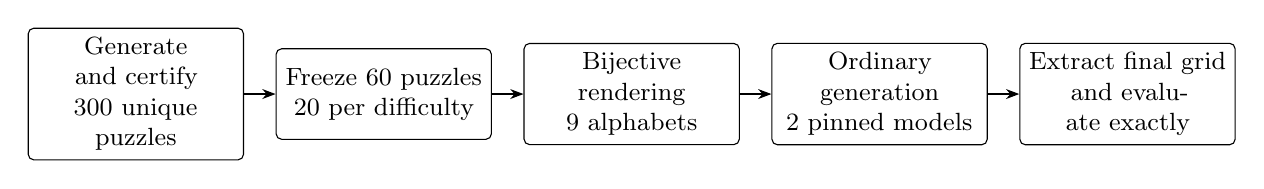
\begin{tikzpicture}[node distance=0.4cm, every node/.style={font=\small}, box/.style={draw,rounded corners=2pt,align=center,minimum height=1.15cm,text width=2.5cm}, >={Stealth}]
\node[box] (a) {Generate and certify\\300 unique puzzles};
\node[box,right=of a] (b) {Freeze 60 puzzles\\20 per difficulty};
\node[box,right=of b] (c) {Bijective rendering\\9 alphabets};
\node[box,right=of c] (d) {Ordinary generation\\2 pinned models};
\node[box,right=of d] (e) {Extract final grid\\and evaluate exactly};
\draw[->] (a)--(b); \draw[->] (b)--(c); \draw[->] (c)--(d); \draw[->] (d)--(e);
\end{tikzpicture}
\caption{Main evaluation pipeline. Each model produces 540 answers for the same 60 puzzles. The exact solver certifies data and supplies reference solutions, but is not available to the model during main inference.}
\label{fig:pipeline}
\end{figure*}

\subsection{Dataset construction and difficulty}
The seeded generator produces a complete valid grid and removes clues in seeded order, retaining a removal only when an exact solver confirms that exactly one solution remains. Candidates are rejected if their measured difficulty does not match the requested tier. Puzzle hashes exclude exact duplicate grids. This procedure does not deduplicate all Sudoku symmetries or prove absence from model pretraining.

Difficulty is assigned by a fixed deterministic technique procedure. Easy puzzles complete with singles. Medium puzzles complete using at least one intermediate technique: naked pairs, hidden pairs, pointing pairs, or box-line reductions. Hard puzzles cause that procedure to stall and are then completed by reference search. These labels describe the registered procedure, not validated human difficulty or a proof that every solver needs search. Table~\ref{tab:dataset} reports actual accepted clue ranges.

\begin{table}[t]
\centering\small
\begin{tabular}{lrrrr}
\toprule
Tier & Pool & Main & Clues & Median\\
\midrule
Easy & 100 & 20 & 40--46 & 43\\
Medium & 100 & 20 & 24--28 & 26\\
Hard & 100 & 20 & 23--27 & 25\\
\bottomrule
\end{tabular}
\caption{Certified dataset and frozen main sample. Clue statistics describe all 100 accepted puzzles in each tier.}
\label{tab:dataset}
\end{table}

Each record stores its puzzle, solution, clue mask, seed, hash, uniqueness certificate, and difficulty certificate. A local audit re-executes the registered uniqueness and difficulty checks, verifies the manifest, and checks clue consistency and duplicate records. Independent grid checks separately validate saved responses. The uniqueness audit reuses the registered solver rather than an independently implemented SAT solver.

\subsection{Sampling and symbolic transformations}
Selection ranks puzzle IDs using SHA-256 with the master seed, a selection namespace, and tier. The pilot contains five puzzles per tier. Main selection excludes pilot puzzles and selects 20 per tier. The mechanism subset contains five main puzzles per tier, and the ablation subset contains three mechanism puzzles per tier. These follow-ups are nested within the main sample, not independent held-out evaluations.

The nine main alphabets are ASCII Arabic digits, Devanagari numerals, Bengali numerals, uppercase Latin, lowercase Latin, Greek letters, abstract symbols, color emoji, and nonce labels. Each is an ordered set of nine distinct nonempty labels, stored in Unicode NFC form. Position in that set defines the abstract value. Encoding round-trip checks verify that both the transformed puzzle and solution decode to their canonical originals. Appendix~\ref{app:alphabets} gives the exact symbol definitions.

All conditions preserve the clue positions, empty cells, and constraints. The empty marker is a period. The natural-language instructions remain English. Nonce labels are arbitrary strings, not labels proved semantically neutral across every language. The main intervention jointly changes several surface properties, so it measures representation choice rather than isolating script familiarity, tokenization, or visual association.

\subsection{Prompting and final-answer evaluation}
The main prompt lists the alphabet, states the row, column, box, and clue-preservation rules, and instructs consistent label use. It requests exactly nine lines of nine single-space-separated symbols, without prose or Markdown. The user message uses the checkpoint's chat template and contains no examples or solver-generated hints. Appendix~\ref{app:prompt} reproduces a complete saved main prompt.

We use ordinary generation rather than grammar-constrained or Sudoku-constrained decoding. The backend extracts GPT-OSS's Harmony final channel and removes Qwen's thinking-tag portion. Hidden reasoning consumes generation allowance but is excluded from scoring and analysis. The evaluator checks exact structure and alphabet membership, decodes the grid, verifies all clues and 27 units, and compares it with the unique reference solution. Matching shape alone is insufficient.

Error labels may overlap. We therefore report exclusive outcomes in priority order: operational failure, correct answer, incorrect length-stopped generation, other output error, and remaining incorrect parseable grid. Other output errors include format, invalid-symbol, Unicode, missing-answer, and refusal errors. The grid category includes completed Sudoku grids that violate the original clues. Parseability, clue preservation, and all-unit validity are also reported independently, with parseable grids as the denominator for the latter two properties.

\subsection{Controlled follow-ups}
Both models complete every follow-up on the same nested puzzle sets. The input/output cross uses Arabic-to-Arabic, Greek-to-Greek, Greek-to-Arabic, and Arabic-to-Greek on 15 puzzles. Same-alphabet baselines reuse each model's matching main answers. Cross prompts explicitly provide mappings. Five controls per puzzle test Greek copying, short translation, coordinate retrieval, symbol counting, and conversion of a supplied completed grid. Each model has 135 outcomes, including 30 reused baselines and 105 new calls.

The token-length study constructs nine-label alphabets with one, two, or three tokenizer tokens per label, checking isolation and leading-space tokenization. Each model uses its own pinned tokenizer, so the visible label sets need not match across models. Each makes 45 new calls on the same 15 puzzles. Recorded covariates include prompt tokens, clue tokens, UTF-8 bytes, and code points. Label identity changes with bin, limiting causal interpretation.

The binding study evaluates 11 assignments on the same 15 puzzles: six assignments of uppercase labels, ordinary and permuted digits, ordinary and permuted number words, and nonce labels. A permutation changes how the canonical grid is rendered. It is not a test of obeying an explicit conflicting arithmetic definition. Three conditions reuse main outputs.

The prompt/output study evaluates 19 variants on nine puzzles. It varies rule detail, mapping instructions, output format, empty markers, and letter case. Alternative formats are normalized according to their requested contract before checking Sudoku validity. Four condition names generate identical default prompts but have separate generations, permitting a direct check of response variation.

The revision study uses nine puzzles in Arabic, Greek, and emoji, giving 27 shared initial main answers. Branches retain one pass, request one self-revision, request two successive self-revisions, or request checker-guided revision only for an incorrect initial answer. The checker reports clue, unit, or format violations without supplying the complete solution. Its correctness-based stopping rule gives it a selection advantage over unconditional self-revision. Costs include the initial generation and every subsequent call.

\section{Experimental Setup}
\subsection{Models and inference}
We evaluate the pinned \texttt{openai/gpt-oss-120b} checkpoint \citep{openai2025gptoss} and \texttt{Qwen/Qwen3.8-27B-FP8} \citep{qwen2026card}. Both were selected for local deployment feasibility and observed readiness. No model is trained or fine-tuned in this study. GPT-OSS is a mixture-of-experts checkpoint, while Qwen's language component is dense. Their parameter labels do not establish comparable active computation.

\begin{table}[t]
\centering\small
\begin{tabular}{p{2.55cm}rr}
\toprule
Setting & GPT-OSS & Qwen\\
\midrule
Reasoning effort & high & xhigh\\
Temperature / top-$p$ & 1 / 1 & 1 / 1\\
Context ceiling & 131,072 & 131,072\\
Output ceiling & 131,072 & 131,072\\
Host RAM (GB) & 192 & 96\\
Main hash shards & 6 & 12\\
\bottomrule
\end{tabular}
\caption{Main deployed configurations. Both use one H100, 12 CPUs, vLLM, seed 20260826, tensor parallelism 1, and one concurrent sequence per backend. Token ceilings are in tokenizer tokens.}
\label{tab:settings}
\end{table}

Table~\ref{tab:settings} summarizes the effective settings. Qwen thinking is enabled. Provider-specific effort labels are not equal-compute guarantees. Prompt and generation share the total context, so the allowed output is reduced by prompt length. Hidden reasoning and the final grid share this allowance. There is no demonstrated 600-second local per-request timeout or reserved final-answer phase. Matched settings also differ from some vendor-recommended defaults.

\subsection{Readiness, execution, and baselines}
Both models solve all five qualification requests without operational failures. GPT-OSS's qualification threshold is 5/5, while Qwen's approved threshold is at least 3/5 easy with no operational failures. The qualification puzzles in the verified captures are disjoint from pilot and main samples. The 60-request pilot scores are 47/60 for GPT-OSS and 54/60 for Qwen. Pilot results establish feasibility and are not pooled into main accuracy.

Main inference runs through Slurm on H100 compute nodes. Deterministic hash shards partition requests for scheduling. Append-only records are flushed and synchronized to storage. Resumption skips saved request IDs, and frozen manifests guard against protocol changes. A completion claim requires marker/count agreement and a matching request digest. Both models satisfy these checks for all 540 main requests.

Arabic digits are the within-model representation baseline. Cross-model comparisons pair the same puzzle and alphabet. Exact solving supplies reference data but is not a model inference baseline. Mechanism conditions test specific behavioral contrasts. They are not comparisons with prior papers' reported accuracies on different datasets.

Latency measures an individual generation call, excluding checkpoint loading and queueing. Job wall-time includes initialization and teardown. A Slurm timeout and a saved request-level operational error are different events. Resumed parts contribute one saved outcome per request rather than independent replicates.

\subsection{Metrics and statistical analysis}
We report numerators, denominators, accuracy, exclusive failures, parseability, clue preservation, unit validity, and mean and median generation latency. Arabic-baseline retention is
\begin{equation}
 R_{ma}=\frac{\sum_p Y_{pm,\mathrm{Arabic}}Y_{pma}}
 {\sum_p Y_{pm,\mathrm{Arabic}}}.
\end{equation}
We also count Arabic-only and alphabet-only successes. Retention alone omits gains from transformed representations.

Paired alphabet comparisons use the exact two-sided McNemar test on discordant puzzle outcomes. Holm correction covers eight Arabic-baseline comparisons separately within each model. The global model difference uses a stratified puzzle-cluster bootstrap with 10,000 replicates and seed 20260930. Each replicate resamples 20 puzzles within each tier, preserving all nine alphabets per puzzle. Holm adjustment and this bootstrap are exploratory report analyses added after capture, not amendments to the frozen protocol. The interval measures variation over puzzle clusters, not within-prompt sampling variance.

\section{Results and Discussion}
\subsection{Representation accuracy and retention}
\paragraph{Objective.} We test how realized accuracy and Arabic-correct puzzle retention change under bijective relabeling.
\paragraph{Findings.} Table~\ref{tab:representation} reports every alphabet. GPT-OSS ranges from 37/60 for Greek to 45/60 for Arabic and uppercase Latin. Qwen ranges from 48/60 for nonce labels to 56/60 for Devanagari. The observed alphabet ordering is model-dependent, but these ranks do not establish a reliable model-by-alphabet interaction.

\begin{table}[t]
\centering\small
\begin{tabular}{lrr}
\toprule
Alphabet & GPT-OSS & Qwen\\
\midrule
Arabic digits & 45/60 & 53/60\\
Devanagari & 39/60 & 56/60\\
Bengali & 43/60 & 53/60\\
Uppercase Latin & 45/60 & 55/60\\
Lowercase Latin & 44/60 & 51/60\\
Greek & 37/60 & 51/60\\
Abstract symbols & 38/60 & 51/60\\
Color emoji & 38/60 & 54/60\\
Nonce labels & 43/60 & 48/60\\
\bottomrule
\end{tabular}
\caption{Correct answers by alphabet on the same 60 puzzles. Counts are paired within and across models.}
\label{tab:representation}
\end{table}

GPT-OSS's Arabic-versus-Greek comparison has an unadjusted exact $p=0.0215$, but its Holm-adjusted value is $0.1719$. All other adjusted GPT-OSS values and all adjusted Qwen values are 1.0. Thus no alphabet comparison survives adjustment at $\alpha=0.05$. This does not prove invariance or equivalence. It limits claims of a reliably better or worse alphabet from this sample.

Retention reveals exchanges of successful puzzles that marginal accuracy hides. GPT-OSS scores 45/60 in both Arabic and uppercase Latin, but only 36 of the 45 Arabic successes remain correct in uppercase. Nine puzzles succeed only in Arabic and nine only in uppercase. For Qwen, Devanagari retains 51/53 Arabic successes, loses two, and gains five. Appendix~\ref{app:stats} gives all paired counts and tests. With one sampled answer per cell, these exchanges cannot be separated completely from generation variation.

\subsection{Output compliance and grid errors}
\paragraph{Objective.} We distinguish failures to produce a usable answer from failures of the completed grid.
\paragraph{Findings.} Table~\ref{tab:errors} shows that neither model has a saved request-level operational failure. Both have 24 incorrect length-stopped generations. Qwen produces fewer remaining incorrect grids and fewer other output errors.

\begin{table}[t]
\centering\small
\begin{tabular}{lrr}
\toprule
Exclusive outcome & GPT-OSS & Qwen\\
\midrule
Correct & 372 & 472\\
Incorrect parseable grid & 96 & 33\\
Incorrect truncation & 24 & 24\\
Other output error & 48 & 11\\
Operational failure & 0 & 0\\
\midrule
Total & 540 & 540\\
\bottomrule
\end{tabular}
\caption{Exclusive main outcomes. Incorrect parseable grids in this partition exclude length-stopped failures and can include valid Sudoku grids that change clues.}
\label{tab:errors}
\end{table}

The independent checker parses 468/540 GPT-OSS outputs (86.7\%) and 505/540 Qwen outputs (93.5\%). Among parseable grids, GPT-OSS preserves all clues in 454/468 and satisfies all Sudoku units in 377/468. Qwen preserves all clues in 488/505 and satisfies all units in 487/505. Fourteen GPT-OSS grids and 17 Qwen grids change givens. Five GPT-OSS and 15 Qwen outputs are valid completed Sudoku grids but fail the original clues. Unit validity therefore cannot replace full puzzle correctness.

Truncations account for 14.3\% of GPT-OSS failures and 35.3\% of Qwen failures. Even a hypothetical perfect repair of every truncated answer would yield only 396/540 and 496/540 correct, respectively. These are arithmetic bounds, not measured reruns. They demonstrate that truncation alone cannot explain all failures. The primary accuracy retains the full request denominator rather than conditioning on parseability.


\subsection{Tokenization: measurements and intervention}\label{sec:tokenization}
\paragraph{Objective.} We test whether segmentation and prompt length sufficiently explain the observed alphabet outcomes.
\paragraph{Measurements.} Each completed registry records token IDs for all 81 labels, plus alphabet-row and puzzle-prompt token counts. Table~\ref{tab:tokenization} combines these with backend input counts for the 60 main puzzles. Both tokenizers encode Arabic digits as one token in isolation and two after a space. GPT-OSS encodes Greek labels as one isolated token and one or two after a space. Qwen uses one in both positions. Qwen's Indic labels use two in isolation and three after a space, unlike GPT-OSS's one and two.

\begin{table*}[t]
\centering\small
\begin{tabular}{llrrrrr}
\toprule
Model & Alphabet & Isolated & Leading space & Alphabet row & Mean input & Correct\\
\midrule
GPT-OSS & Arabic & 1 & 2 & 17 & 287.2 & 45/60 \\
GPT-OSS & Devanagari & 1 & 2 & 17 & 287.2 & 39/60 \\
GPT-OSS & Bengali & 1 & 2 & 17 & 287.2 & 43/60 \\
GPT-OSS & Uppercase Latin & 1 & 1 & 9 & 251.5 & 45/60 \\
GPT-OSS & Lowercase Latin & 1 & 1 & 9 & 251.5 & 44/60 \\
GPT-OSS & Greek & 1 & 1--2 & 10 & 255.5 & 37/60 \\
GPT-OSS & Abstract & 1 & 1--2 & 10 & 255.6 & 38/60 \\
GPT-OSS & Emoji & 2--3 & 2--3 & 23 & 314.5 & 38/60 \\
GPT-OSS & Nonce & 2 & 2 & 18 & 291.8 & 43/60 \\
Qwen & Arabic & 1 & 2 & 17 & 288.7 & 53/60 \\
Qwen & Devanagari & 2 & 3 & 26 & 329.1 & 56/60 \\
Qwen & Bengali & 2 & 3 & 26 & 329.1 & 53/60 \\
Qwen & Uppercase Latin & 1 & 1 & 9 & 253.0 & 55/60 \\
Qwen & Lowercase Latin & 1 & 1 & 9 & 253.0 & 51/60 \\
Qwen & Greek & 1 & 1 & 9 & 253.0 & 51/60 \\
Qwen & Abstract & 1--2 & 1--2 & 11 & 261.7 & 51/60 \\
Qwen & Emoji & 3 & 2--3 & 26 & 326.6 & 54/60 \\
Qwen & Nonce & 2 & 2 & 18 & 293.3 & 48/60 \\
\bottomrule
\end{tabular}

\caption{Measured token counts and main outcomes for both models. Label columns give ranges over nine labels. Alphabet row is the complete space-separated list. Mean input includes chat-template overhead and averages 60 main puzzles. Registry user-message counts exclude that overhead.}
\label{tab:tokenization}
\end{table*}

The profiles show that token count does not completely describe the realized differences. For GPT-OSS, Arabic, Devanagari, and Bengali have identical count profiles but score 45/60, 39/60, and 43/60. Greek inputs are shorter than Arabic inputs but score 37/60. For Qwen, Devanagari and Bengali have identical profiles but score 56/60 and 53/60. Uppercase Latin, lowercase Latin, and Greek also have identical counts but score 55/60, 51/60, and 51/60. Token identity and training can matter when counts match. These observations do not establish causal script effects or stable accuracy differences.

Multi-token representation alone does not demonstrate text corruption or inability to emit a label. Every main alphabet has correctly generated full solutions, which necessarily contain all nine output labels. Thus complete inability to produce one of these alphabets cannot explain its failures. This does not imply that every response handles its symbols correctly. The registry records segmentation, not a causal diagnosis of individual invalid-symbol errors.

\paragraph{Token-length intervention.} GPT-OSS's one-, two-, and three-token alphabets solve 9/15, 13/15, and 10/15. Qwen's corresponding constructions solve 12/15, 11/15, and 14/15 (Table~\ref{tab:mechanisms}). Tier totals are 15/15 easy, 13/15 medium, and 4/15 hard for GPT-OSS, versus 14/15, 15/15, and 8/15 for Qwen. Truncations number five and two. Both patterns are non-monotonic, with different highest-scoring bins. They do not support a universal shorter-label advantage.

Both registered multivariable fits have singular information matrices, with token, byte, code-point, and prompt-length measures co-varying in their constructions. Label identities also change between bins and models. No independent token-length coefficient is identified. Tokenization remains a candidate contributor, but these data do not identify it as the cause of the accuracy ranking.

Table~\ref{tab:runtime_tokens} in Appendix~\ref{app:stats} reports input tokens, generated tokens, unparseable outputs, and truncations by alphabet for both main models. Generated-token counts include hidden reasoning and the final answer. They are not measurements of final-grid length alone. An unparseable output is an observed output-contract failure, not evidence that the local parser corrupted otherwise valid text.

\subsection{Simple symbol handling versus integrated solving}
\paragraph{Objective.} We distinguish basic input/output operations from solving while converting between alphabets.
\paragraph{Findings.} Both models pass all 75 no-Sudoku controls, including copying, translation, retrieval, counting, and supplied-grid conversion. GPT-OSS's Sudoku conditions score 12/15, 12/15, 10/15, and 11/15 in same-Arabic, same-Greek, Greek-to-Arabic, and Arabic-to-Greek order. Qwen scores 13/15, 11/15, 11/15, and 10/15 (Table~\ref{tab:mechanisms}). Both solve 45/60 Sudoku outcomes, with identical tier totals of 19/20 easy, 18/20 medium, and 8/20 hard. Equal totals do not imply identical successful cells. Truncations number two for GPT-OSS and six for Qwen.

\begin{table}[t]
\centering\small
\begin{tabular}{lrr}
\toprule
Condition & GPT-OSS & Qwen\\
\midrule
Arabic $\rightarrow$ Arabic & 12/15 & 13/15\\
Greek $\rightarrow$ Greek & 12/15 & 11/15\\
Greek $\rightarrow$ Arabic & 10/15 & 11/15\\
Arabic $\rightarrow$ Greek & 11/15 & 10/15\\
No-Sudoku controls & 75/75 & 75/75\\
\midrule
One-token labels & 9/15 & 12/15\\
Two-token labels & 13/15 & 11/15\\
Three-token labels & 10/15 & 14/15\\
\bottomrule
\end{tabular}
\caption{Both models' input/output and token-length conditions. Controls are not Sudoku solves. Same-alphabet baselines reuse main outcomes. Token-length alphabets are tokenizer-specific.}
\label{tab:mechanisms}
\end{table}

These results weaken a broad explanation based on inability to copy or translate the tested labels. GPT-OSS's same-alphabet baselines are equal. Qwen's Greek-to-Arabic score equals its Greek-to-Greek score, so Arabic output does not improve this aggregate. Cross prompts introduce mappings and extra instructions, preventing pure input/output attribution. Successful short controls are weaker evidence than unrestricted symbol competence during long solving.

The main benchmark uses nonzero Arabic baselines in every tier: GPT-OSS solves 20/20 easy, 14/20 medium, and 11/20 hard Arabic puzzles. Conditional retention therefore evaluates changed notation where baseline successes exist, rather than interpreting a floor score as an invariance failure. Nevertheless, the nested mechanism subset is small and its paired outcomes remain sampled observations.

\subsection{Label assignment and semantic associations}
\paragraph{Objective.} We test whether changing assignments within or across label families affects realized outcomes while keeping the abstract Sudoku fixed.
\paragraph{Findings.} GPT-OSS solves 124/165 outcomes. Ordinary digits, ordinary number words, and nonce labels each score 12/15, while permuted digits and words score 10/15. Qwen solves 147/165. Ordinary and permuted digits score 13/15 and 15/15, ordinary and permuted words 12/15 and 9/15, and nonce labels 14/15. Uppercase assignments span 10/15--13/15 for GPT-OSS and 12/15--15/15 for Qwen. Appendix~\ref{app:followups} reports all conditions and tiers.

A permutation changes which label renders each canonical value, not an instruction to accept a false arithmetic definition. Both models lose answers under permuted number words, but digit permutations have opposite score directions. This contradicts a universal permutation penalty. Small fixed-assignment contrasts do not establish semantic interference. Label identity, selected puzzles, and generation variability remain alternatives.

\subsection{Prompt and output-format burden}
\paragraph{Objective.} We examine whether rule wording, explicit mappings, output format, empty markers, or case offer a stable account of failures.
\paragraph{Findings.} The 19 ablations produce 103/171 correct GPT-OSS outcomes and 130/171 Qwen outcomes. Digit mapping and uppercase nonce score 8/9 for GPT-OSS and 9/9 for Qwen. Qwen's minimal-rules condition also scores 9/9. Compact rows score 3/9 and 2/9, and string81 scores 3/9 and 4/9. Alternate formats use their own contracts. Appendix~\ref{app:followups} gives all variants and failure categories.

Four identical-default-prompt conditions score 5/9, 6/9, 5/9, and 7/9 for GPT-OSS. Qwen's four conditions have the same binary success set, 7/9, but this does not establish identical erroneous grids or deterministic future inference. GPT-OSS's variation occurs despite the fixed recorded sampling seed, and these records do not separate stochastic effects from runtime nondeterminism. Small ablation differences cannot automatically be attributed to wording.

Output compliance and correctness are separable. Qwen has 155 parseable ablation outputs, of which 147 satisfy all units but only 137 preserve clues. Its 130 correct outputs must not be replaced by the unit-valid count. Shared weak compact-row scores and high digit-mapping scores motivate further testing, not a proven interface mechanism. No variant is uniformly superior across all cells, and selecting the best on nine puzzles would not validate a new prompt.

\subsection{Verification, self-revision, and recoverable errors}
\paragraph{Objective.} We determine which incorrect shared initial answers can be corrected by further generation or deterministic violation feedback.
\paragraph{Findings.} Table~\ref{tab:revision} reports outcomes and cumulative generation cost. GPT-OSS's one- and two-revision branches fix one and five initial failures, with no observed regression. Qwen's one revision fixes three of four failures and reaches 26/27. Two revisions end at 23/27, with two fixes and two regressions relative to the initial answer. More revision therefore does not consistently improve correctness. Mean cumulative time rises from 312.25 to 610.69 seconds for GPT-OSS's two-revision branch and from 561.28 to 788.07 for Qwen's.

\begin{table*}[t]
\centering\small
\begin{tabular}{llrrrrr}
\toprule
Model & Arm & Correct & Fixed & Regressed & New calls & Mean total (s)\\
\midrule
GPT-OSS & one pass & 18/27 & 0 & 0 & 0 & 312.25\\
GPT-OSS & one self revision & 19/27 & 1 & 0 & 27 & 482.60\\
GPT-OSS & two self revisions & 23/27 & 5 & 0 & 54 & 610.69\\
GPT-OSS & checker guided revision & 22/27 & 4 & 0 & 9 & 476.68\\
Qwen & one pass & 23/27 & 0 & 0 & 0 & 561.28\\
Qwen & one self revision & 26/27 & 3 & 0 & 27 & 725.74\\
Qwen & two self revisions & 23/27 & 2 & 2 & 54 & 788.07\\
Qwen & checker guided revision & 26/27 & 3 & 0 & 4 & 718.79\\
\bottomrule
\end{tabular}

\caption{Revision from 27 shared initials per model on nine puzzles in three alphabets. New calls exclude the initial solve; cumulative latency includes it. Checker revision calls only on initially incorrect answers: nine for GPT-OSS and four for Qwen.}
\label{tab:revision}
\end{table*}

Checker feedback repairs 4/9 GPT-OSS and 3/4 Qwen initial failures, reaching 22/27 and 26/27 overall. It leaves correct initials untouched, so its absence of regressions partly follows from selection. Generic revision can damage a correct answer, as Qwen's two-revision outcomes demonstrate. Corrections do not localize the original error to decoding, binding, solving, or final emission.

No equal-compute independent-resampling baseline is included. Revision gains can reflect additional computation, a new sampling opportunity, explicit checking, or feedback information. The 27 cells are clustered within nine puzzles and do not establish a universal self-correction benefit.

\subsection{What explains the observed performance?}
The main benchmark describes variation across equivalent symbol systems. The follow-ups assess candidate explanations rather than assuming that every change demonstrates a loss of abstract reasoning. Table~\ref{tab:explanations} brings the evidence together.

\begin{table*}[t]
\centering\small
\begin{tabular}{p{3.0cm}p{5.6cm}p{6.0cm}}
\toprule
Candidate explanation & Relevant two-model evidence & Supported interpretation and remaining uncertainty\\
\midrule
Longer token sequences & Matched profiles with different scores; GPT-OSS bins 9/15, 13/15, 10/15 and Qwen bins 12/15, 11/15, 14/15 & Neither pattern is monotonic. Both regressions are singular. Counts do not identify a causal token effect.\\
\addlinespace
Basic symbol decoding or emission & Each passes 75/75 controls but solves 45/60 input/output Sudoku conditions; each solves examples in every main alphabet & General inability to handle tested labels is insufficient. Integrated solving can still fail.\\
\addlinespace
Binding or semantic interference & Permuted words lose answers in both; digit scores fall from 12 to 10 for GPT-OSS but rise from 13 to 15 for Qwen & No universal permutation penalty is established. Small fixed-assignment contrasts do not isolate semantics.\\
\addlinespace
Output format or resource limits & GPT-OSS has 72 output/length failures and 96 incorrect grids; Qwen has 35 and 33 respectively & Output failures contribute but cannot explain all failures. Truncation is not an operational failure.\\
\addlinespace
Prompt choice or generation variation & GPT-OSS's identical-prompt totals vary from 5/9 to 7/9; Qwen's are all 7/9 & Equal aggregates do not establish identical cells. Small differences cannot be attributed solely to wording.\\
\addlinespace
Insufficient checking of an answer & Two revisions fix five GPT-OSS initials, but Qwen has two fixes and two regressions; checker feedback improves both & More revision is not universally better. Extra compute, selection, and feedback remain confounded.\\
\bottomrule
\end{tabular}
\caption{Evidence-based explanation map. These tests constrain simple accounts of the observed behavior without identifying a single causal mechanism.}
\label{tab:explanations}
\end{table*}

First, there is no adequate token-count-only explanation: matched counts coexist with different saved outcomes, and shorter constructions do not consistently solve more puzzles. Second, simple symbol-handling competence does not guarantee reliable integrated solving. Third, formatting and length limits account for some failures, while incorrect parseable grids show that fixing output shape alone would be insufficient. Assignment tests and revision provide further behavioral evidence, but not a unique causal localization.

Generation variability also limits interpretation of the main symbol changes. With one answer per cell and no alphabet contrast surviving correction, the study does not establish a reliable harmful alphabet or a general familiarity hierarchy. It instead measures the observed success exchanges and uses controls to reject overly simple explanations. Repeated generations and independently varied representation properties would be needed to estimate stable alphabet effects and distinguish them from sampling variation.

This account complements symbol-tuning and equivariant-model research: enforced symmetry is a design property, whereas our evaluation measures realized behavior. It follows cautions about perturbation comparisons and intrinsic self-correction \citep{dlugosz2026earnest,huang2024selfcorrect}. The two-model evidence supports bounded behavioral conclusions, not a reconstruction of hidden reasoning or a general claim that language models lack abstract reasoning.

\section{Conclusion}
We evaluated symbol-set variation on 60 certified Sudoku puzzles in nine bijective alphabets for two local reasoning models. The main results showed different realized accuracies and exchanges of successful puzzles across equivalent representations, but no Arabic-baseline comparison survived Holm adjustment. These findings describe the tested outcomes rather than establish a reliable ordering of alphabets.

Both models' completed tokenizer profiles and follow-ups constrained explanations. Matched count profiles coexisted with different outcomes, constructed token lengths were non-monotonic, and perfect simple controls did not guarantee solving. Permuted words reduced both scores, while digit permutations had opposite directions. Two revisions improved GPT-OSS, but Qwen lost its one-revision gain and regressed on two initially correct answers. Formatting and truncation contributed without accounting for every incorrect grid. These shared and differing outcomes left causal localization unresolved. Repeated generations, independently varied token properties, and equal-compute revision controls remain next steps.

\section*{Limitations}
The main sample contains 60 underlying puzzles, not 540 independent puzzles. There are only 20 puzzles per alphabet/difficulty cell, 15 per mechanism condition, and nine underlying puzzles in the ablation and revision studies. One generation per main cell does not estimate within-prompt sampling variance. Lack of a significant corrected comparison is not evidence of equivalence.

The dataset is procedurally generated and difficulty is relative to a fixed technique procedure. Exact duplicate exclusion does not exclude symmetric puzzles, and no human difficulty study or pretraining-contamination audit is available. Mechanism samples are nested within main puzzles and reuse some main baselines. Reused records must not be interpreted as independent replications.

Only two feasibility-screened checkpoints are evaluated. Their architectures, quantization, tokenizers, reasoning controls, and effective compute differ. Matching context ceilings and sampling parameters does not equalize resources or guarantee vendor-optimal inference. Model-level environment provenance is available, but separate environment capture for every shard is not established.

Representation changes conflate label identity, script, semantics, tokenization, and prompt length. Both token-length regressions are singular, cross prompts add mapping burden, and revision lacks equal-compute controls. Input/output controls cover Greek and Arabic, not every alphabet. Token-length labels are tokenizer-specific rather than identical across models. No fully crossed reasoning-enabled versus reasoning-disabled experiment or separate final-grid token counts are available. Corresponding follow-ups compare two selected configurations, not all language models or unobserved reasoning mechanisms.

\section*{Acknowledgements}
The experiments used the Sharanga computing facility at BITS Pilani.

\paragraph{AI use statement.} An AI assistant was used to draft manuscript text, organize verified experimental evidence, and prepare the LaTeX document. The authors are responsible for reviewing the scientific claims, citations, analyses, and final submission. The experimental model outputs were evaluated as final grids, not used as evidence about their internal reasoning.

\bibliography{references}

\clearpage
\appendix
\section{Full Main Prompt}\label{app:prompt}
The following is the saved Arabic-digit prompt for main puzzle E003. Other alphabets substitute the valid labels and clue symbols. The main prompt is a user message with the checkpoint's own chat template and has no added solver hint.
\begin{Verbatim}[fontsize=\footnotesize,breaklines=true,breakanywhere=true]
Solve the following 9x9 Sudoku.

Valid input symbols:
1 2 3 4 5 6 7 8 9

Rules:
- Every row must contain each valid value exactly once.
- Every column must contain each valid value exactly once.
- Every 3x3 box must contain each valid value exactly once.
- Do not change the given cells.
- The visible symbols are labels; apply the same symbol-value mapping everywhere.

Puzzle:
2 4 . . . 5 1 . 9
7 . . . . 6 . . 5
. 8 . 2 . . . . 7
3 5 2 4 . 7 . . 8
. . 1 . . 3 7 . 2
. 7 4 8 2 1 5 6 .
4 9 3 5 1 2 8 . .
5 . . 6 . . . 9 4
. 2 8 . 4 . . . .

Return only 9 lines of 9 space-separated output symbols.
\end{Verbatim}

\section{Exact Symbol Definitions}\label{app:alphabets}
Table~\ref{tab:alphabets} specifies the nine ordered alphabets. To avoid font-dependent substitution of Indic and emoji glyphs in the PDF, non-Latin labels are given by their Unicode code points. Each listed code point is one label. Greek values are U+03B1, U+03B2, U+03B3, U+03B4, U+03B5, U+03B6, U+03B7, U+03B8, and U+03B9. All main encodings use single spaces and the period empty marker. The exact UTF-8 strings are also in the repository's representation definitions.

\begin{table*}[t]
\centering\small
\begin{tabular}{lp{11.5cm}}
\toprule
Alphabet & Ordered labels for abstract values 1 through 9\\
\midrule
Arabic & \texttt{1 2 3 4 5 6 7 8 9}\\
Devanagari & U+0967 through U+096F, inclusive and ascending\\
Bengali & U+09E7 through U+09EF, inclusive and ascending\\
Uppercase Latin & \texttt{A B C D E F G H I}\\
Lowercase Latin & \texttt{a b c d e f g h i}\\
Greek & U+03B1 through U+03B9, inclusive and ascending\\
Abstract & U+25B3, U+25A1, U+25CB, U+2606, U+00D7, U+2020, U+2021, U+00A7, U+00B6\\
Emoji & U+1F534, U+1F7E0, U+1F7E1, U+1F7E2, U+1F535, U+1F7E3, U+1F7E4, U+26AB, U+26AA\\
Nonce & \texttt{KAV MIP ZOT RUL BEK DAX PEV NUG WIF}\\
\bottomrule
\end{tabular}
\caption{Exact main alphabets. Code-point notation specifies the stored labels rather than relying on the reader's font or emoji renderer.}
\label{tab:alphabets}
\end{table*}

\section{Paired Statistics and Difficulty Results}\label{app:stats}
\begin{table*}[t]
\centering\small
\begin{tabular}{llrrrr}
\toprule
Model & Alphabet & Mean input tokens & Mean generated tokens & Unparseable & Truncated\\
\midrule
GPT-OSS & Arabic & 287.2 & 49942 & 1/60 & 1/60 \\
GPT-OSS & Devanagari & 287.2 & 45393 & 8/60 & 1/60 \\
GPT-OSS & Bengali & 287.2 & 51686 & 9/60 & 2/60 \\
GPT-OSS & Uppercase Latin & 251.5 & 49452 & 3/60 & 2/60 \\
GPT-OSS & Lowercase Latin & 251.5 & 49481 & 5/60 & 2/60 \\
GPT-OSS & Greek & 255.5 & 57255 & 8/60 & 3/60 \\
GPT-OSS & Abstract & 255.6 & 66630 & 16/60 & 7/60 \\
GPT-OSS & Emoji & 314.5 & 60442 & 13/60 & 3/60 \\
GPT-OSS & Nonce & 291.8 & 62524 & 9/60 & 3/60 \\
Qwen & Arabic & 288.7 & 38180 & 4/60 & 4/60 \\
Qwen & Devanagari & 329.1 & 33724 & 3/60 & 2/60 \\
Qwen & Bengali & 329.1 & 40795 & 5/60 & 4/60 \\
Qwen & Uppercase Latin & 253.0 & 37525 & 2/60 & 2/60 \\
Qwen & Lowercase Latin & 253.0 & 42833 & 3/60 & 2/60 \\
Qwen & Greek & 253.0 & 41039 & 1/60 & 1/60 \\
Qwen & Abstract & 261.7 & 40748 & 5/60 & 0/60 \\
Qwen & Emoji & 326.6 & 40810 & 4/60 & 2/60 \\
Qwen & Nonce & 293.3 & 49521 & 8/60 & 7/60 \\
\bottomrule
\end{tabular}

\caption{Main input and generation lengths and output failures by alphabet. Each row contains 60 requests. Input counts include chat-template overhead. Generated tokens include hidden reasoning and the final answer. Unparseability and incorrect truncation overlap and must not be added as exclusive categories.}
\label{tab:runtime_tokens}
\end{table*}
Table~\ref{tab:paired} reports the complete Arabic-baseline comparison family. Let $b$ be Arabic-only successes and $c$ be alphabet-only successes. The exact two-sided test conditions on $b+c$ discordant pairs and uses a binomial probability with parameter $1/2$. Holm correction is applied separately to the eight comparisons for each model. Retention is conditional on 45 Arabic-correct GPT-OSS puzzles or 53 Arabic-correct Qwen puzzles.

\begin{table*}[t]
\centering\small
\begin{tabular}{llrrrrr}
\toprule
Model & Alphabet & Retained & $b$ & $c$ & Exact $p$ & Holm $p$\\
\midrule
GPT-OSS & Abstract & 31/45 & 14 & 7 & 0.1892 & 1.0000\\
& Bengali & 36/45 & 9 & 7 & 0.8036 & 1.0000\\
& Devanagari & 36/45 & 9 & 3 & 0.1460 & 1.0000\\
& Emoji & 32/45 & 13 & 6 & 0.1671 & 1.0000\\
& Greek & 36/45 & 9 & 1 & 0.0215 & 0.1719\\
& Lowercase Latin & 37/45 & 8 & 7 & 1.0000 & 1.0000\\
& Nonce & 36/45 & 9 & 7 & 0.8036 & 1.0000\\
& Uppercase Latin & 36/45 & 9 & 9 & 1.0000 & 1.0000\\
\midrule
Qwen & Abstract & 44/53 & 9 & 7 & 0.8036 & 1.0000\\
& Bengali & 48/53 & 5 & 5 & 1.0000 & 1.0000\\
& Devanagari & 51/53 & 2 & 5 & 0.4531 & 1.0000\\
& Emoji & 48/53 & 5 & 6 & 1.0000 & 1.0000\\
& Greek & 46/53 & 7 & 5 & 0.7744 & 1.0000\\
& Lowercase Latin & 46/53 & 7 & 5 & 0.7744 & 1.0000\\
& Nonce & 43/53 & 10 & 5 & 0.3018 & 1.0000\\
& Uppercase Latin & 49/53 & 4 & 6 & 0.7539 & 1.0000\\
\bottomrule
\end{tabular}
\caption{Paired comparisons against Arabic on 60 puzzles per alphabet and model. No Holm-adjusted value is below 0.05.}
\label{tab:paired}
\end{table*}

The cross-model bootstrap resamples complete nine-alphabet puzzle clusters within each difficulty stratum. It preserves both models' outcomes for every sampled cluster. The percentile interval is exploratory and conditional on the tested data and settings. It is not an unclustered test of 540 independent problems. Table~\ref{tab:tiers} gives the full alphabet-by-tier counts, and Table~\ref{tab:latency} gives difficulty-specific latency.

\begin{table*}[t]
\centering\small
\begin{tabular}{lrrrrrr}
\toprule
& \multicolumn{3}{c}{GPT-OSS} & \multicolumn{3}{c}{Qwen}\\
Alphabet & Easy & Medium & Hard & Easy & Medium & Hard\\
\midrule
Arabic & 20 & 14 & 11 & 20 & 19 & 14\\
Devanagari & 18 & 12 & 9 & 20 & 19 & 17\\
Bengali & 17 & 15 & 11 & 19 & 19 & 15\\
Uppercase Latin & 20 & 15 & 10 & 19 & 18 & 18\\
Lowercase Latin & 20 & 15 & 9 & 19 & 15 & 17\\
Greek & 20 & 11 & 6 & 20 & 17 & 14\\
Abstract & 18 & 10 & 10 & 19 & 17 & 15\\
Emoji & 18 & 13 & 7 & 19 & 20 & 15\\
Nonce & 20 & 16 & 7 & 19 & 16 & 13\\
\bottomrule
\end{tabular}
\caption{Correct main answers out of 20 in every alphabet/difficulty cell.}
\label{tab:tiers}
\end{table*}

\begin{table}[t]
\centering\small
\begin{tabular}{lrr}
\toprule
Tier & GPT-OSS (s) & Qwen (s)\\
\midrule
Easy & 53.48 & 110.10\\
Medium & 372.49 & 605.11\\
Hard & 446.45 & 878.53\\
\bottomrule
\end{tabular}
\caption{Mean main generation latency by tier, excluding queueing and initial checkpoint loading.}
\label{tab:latency}
\end{table}

\section{Secondary Model Comparison}\label{app:models}
Table~\ref{tab:main} shows that Qwen solves 100 more requests than GPT-OSS. The paired outcomes are 338 correct for both, 34 correct only for GPT-OSS, 134 correct only for Qwen, and 34 correct for neither. The Qwen-minus-GPT-OSS difference is 18.52 percentage points, with an exploratory 95\% bootstrap interval of 13.70--23.52 points.

\begin{table}[t]
\centering\small
\begin{tabular}{lrr}
\toprule
Metric & GPT-OSS & Qwen\\
\midrule
Overall correct & 372/540 & 472/540\\
Overall accuracy & 68.9\% & 87.4\%\\
Easy correct & 171/180 & 174/180\\
Medium correct & 121/180 & 160/180\\
Hard correct & 80/180 & 138/180\\
Mean latency (s) & 290.81 & 531.25\\
Median latency (s) & 240.46 & 422.78\\
\bottomrule
\end{tabular}
\caption{Completed main benchmark. Each tier has 20 puzzles in nine alphabets, giving 180 requests rather than 180 independent puzzles.}
\label{tab:main}
\end{table}

The model difference is concentrated beyond the easy tier. Accuracy is 95.0\%, 67.2\%, and 44.4\% for GPT-OSS across easy, medium, and hard, compared with 96.7\%, 88.9\%, and 76.7\% for Qwen. The corresponding descriptive advantages are 1.67, 21.67, and 32.22 points. Qwen's mean generation latency is 1.83 times GPT-OSS's. These are outcomes of the deployed configurations, not evidence that smaller parameter count causes greater reasoning accuracy or that the two systems used equal compute.

\section{Complete Follow-up Results}\label{app:followups}
Tables~\ref{tab:crossfull}--\ref{tab:revisionfull} list every follow-up condition and tier for both models. Each ablation uses nine puzzles, three per tier. Rule, mapping, format, and empty-marker variants generally use Greek. Case variants change the alphabet. Alternative formats are normalized under their own contract.

\begin{table*}[t]
\centering\footnotesize
\begin{tabular}{p{4.4cm}rrrrrrrr}
\toprule
Condition & GPT all & Easy & Medium & Hard & Qwen all & Easy & Medium & Hard\\
\midrule
A arabic to arabic & 12/15 & 5/5 & 5/5 & 2/5 & 13/15 & 5/5 & 5/5 & 3/5\\
B greek to greek & 12/15 & 5/5 & 5/5 & 2/5 & 11/15 & 5/5 & 5/5 & 1/5\\
C greek to arabic & 10/15 & 4/5 & 4/5 & 2/5 & 11/15 & 5/5 & 4/5 & 2/5\\
D arabic to greek & 11/15 & 5/5 & 4/5 & 2/5 & 10/15 & 4/5 & 4/5 & 2/5\\
control coordinate retrieval & 15/15 & 5/5 & 5/5 & 5/5 & 15/15 & 5/5 & 5/5 & 5/5\\
control copy & 15/15 & 5/5 & 5/5 & 5/5 & 15/15 & 5/5 & 5/5 & 5/5\\
control grid conversion & 15/15 & 5/5 & 5/5 & 5/5 & 15/15 & 5/5 & 5/5 & 5/5\\
control mapping translation & 15/15 & 5/5 & 5/5 & 5/5 & 15/15 & 5/5 & 5/5 & 5/5\\
control occurrence count & 15/15 & 5/5 & 5/5 & 5/5 & 15/15 & 5/5 & 5/5 & 5/5\\
\bottomrule
\end{tabular}

\caption{All input/output conditions and difficulty counts. Control conditions do not require Sudoku solving. Each Sudoku tier has five puzzles per condition.}
\label{tab:crossfull}
\end{table*}

\begin{table*}[t]
\centering\footnotesize
\begin{tabular}{p{4.4cm}rrrrrrrr}
\toprule
Condition & GPT all & Easy & Medium & Hard & Qwen all & Easy & Medium & Hard\\
\midrule
neutral 1 tokens & 9/15 & 5/5 & 4/5 & 0/5 & 12/15 & 5/5 & 5/5 & 2/5\\
neutral 2 tokens & 13/15 & 5/5 & 5/5 & 3/5 & 11/15 & 4/5 & 5/5 & 2/5\\
neutral 3 tokens & 10/15 & 5/5 & 4/5 & 1/5 & 14/15 & 5/5 & 5/5 & 4/5\\
\bottomrule
\end{tabular}

\caption{All constructed token-length conditions. Labels differ between tokenizers. Each tier uses five puzzles per condition.}
\label{tab:tokenfull}
\end{table*}

\begin{table*}[t]
\centering\footnotesize
\begin{tabular}{p{4.4cm}rrrrrrrr}
\toprule
Condition & GPT all & Easy & Medium & Hard & Qwen all & Easy & Medium & Hard\\
\midrule
empty dot & 7/9 & 3/3 & 3/3 & 1/3 & 7/9 & 3/3 & 3/3 & 1/3\\
empty underscore & 4/9 & 3/3 & 1/3 & 0/3 & 7/9 & 3/3 & 2/3 & 2/3\\
empty word & 6/9 & 3/3 & 3/3 & 0/3 & 8/9 & 3/3 & 2/3 & 3/3\\
empty zero & 6/9 & 3/3 & 3/3 & 0/3 & 6/9 & 3/3 & 2/3 & 1/3\\
latin lowercase & 7/9 & 3/3 & 3/3 & 1/3 & 7/9 & 3/3 & 2/3 & 2/3\\
latin uppercase & 5/9 & 3/3 & 2/3 & 0/3 & 8/9 & 2/3 & 3/3 & 3/3\\
mapping alphabet only & 6/9 & 3/3 & 2/3 & 1/3 & 7/9 & 3/3 & 3/3 & 1/3\\
mapping to abstract & 5/9 & 3/3 & 2/3 & 0/3 & 4/9 & 3/3 & 0/3 & 1/3\\
mapping to digits & 8/9 & 3/3 & 3/3 & 2/3 & 9/9 & 3/3 & 3/3 & 3/3\\
nonce lowercase & 4/9 & 3/3 & 1/3 & 0/3 & 8/9 & 3/3 & 2/3 & 3/3\\
nonce uppercase & 8/9 & 3/3 & 3/3 & 2/3 & 9/9 & 3/3 & 3/3 & 3/3\\
output compact & 3/9 & 2/3 & 1/3 & 0/3 & 2/9 & 1/3 & 0/3 & 1/3\\
output json & 5/9 & 3/3 & 1/3 & 1/3 & 7/9 & 3/3 & 3/3 & 1/3\\
output spaced & 5/9 & 3/3 & 1/3 & 1/3 & 7/9 & 3/3 & 3/3 & 1/3\\
output string81 & 3/9 & 2/3 & 1/3 & 0/3 & 4/9 & 1/3 & 2/3 & 1/3\\
rules constraints alphabet & 5/9 & 3/3 & 2/3 & 0/3 & 7/9 & 2/3 & 2/3 & 3/3\\
rules explicit constraints & 6/9 & 3/3 & 2/3 & 1/3 & 7/9 & 3/3 & 2/3 & 2/3\\
rules fully explicit & 5/9 & 3/3 & 1/3 & 1/3 & 7/9 & 3/3 & 3/3 & 1/3\\
rules minimal & 5/9 & 3/3 & 2/3 & 0/3 & 9/9 & 3/3 & 3/3 & 3/3\\
\bottomrule
\end{tabular}

\caption{All 19 ablations and difficulty counts. Fully explicit rules, alphabet-only mapping, spaced output, and the period empty marker generate identical default prompts but independent outcome records.}
\label{tab:ablation}
\end{table*}

Table~\ref{tab:bindingfull} gives all binding assignments. Standard uppercase, ordinary digits, and nonce labels reuse 45 matching main records. The remaining 120 records are new calls. The input/output experiment similarly contains 30 reused main baselines, 30 new cross calls, and 75 new controls. The token-length and ablation studies contain 45 and 171 fresh calls, respectively. These counts separate records from additional inference.

\begin{table*}[t]
\centering\footnotesize
\begin{tabular}{p{4.4cm}rrrrrrrr}
\toprule
Condition & GPT all & Easy & Medium & Hard & Qwen all & Easy & Medium & Hard\\
\midrule
digits ordinary & 12/15 & 5/5 & 5/5 & 2/5 & 13/15 & 5/5 & 5/5 & 3/5\\
digits permuted & 10/15 & 5/5 & 4/5 & 1/5 & 15/15 & 5/5 & 5/5 & 5/5\\
nonce neutral & 12/15 & 5/5 & 5/5 & 2/5 & 14/15 & 4/5 & 5/5 & 5/5\\
number words conflicting & 10/15 & 5/5 & 4/5 & 1/5 & 9/15 & 2/5 & 4/5 & 3/5\\
number words ordinary & 12/15 & 5/5 & 4/5 & 3/5 & 12/15 & 5/5 & 4/5 & 3/5\\
uppercase random 1 & 11/15 & 5/5 & 5/5 & 1/5 & 12/15 & 5/5 & 4/5 & 3/5\\
uppercase random 2 & 11/15 & 5/5 & 5/5 & 1/5 & 15/15 & 5/5 & 5/5 & 5/5\\
uppercase random 3 & 13/15 & 5/5 & 5/5 & 3/5 & 13/15 & 5/5 & 4/5 & 4/5\\
uppercase random 4 & 12/15 & 5/5 & 5/5 & 2/5 & 15/15 & 5/5 & 5/5 & 5/5\\
uppercase random 5 & 10/15 & 5/5 & 4/5 & 1/5 & 15/15 & 5/5 & 5/5 & 5/5\\
uppercase standard & 11/15 & 5/5 & 4/5 & 2/5 & 14/15 & 4/5 & 5/5 & 5/5\\
\bottomrule
\end{tabular}

\caption{All binding conditions for both models. Permutations are seeded and fixed per condition. Each tier contains five puzzles.}
\label{tab:bindingfull}
\end{table*}

\begin{table*}[t]
\centering\footnotesize
\begin{tabular}{p{4.4cm}rrrrrrrr}
\toprule
Condition & GPT all & Easy & Medium & Hard & Qwen all & Easy & Medium & Hard\\
\midrule
arabic digits: checker guided revision & 8/9 & 3/3 & 3/3 & 2/3 & 9/9 & 3/3 & 3/3 & 3/3\\
arabic digits: one pass & 7/9 & 3/3 & 3/3 & 1/3 & 7/9 & 3/3 & 3/3 & 1/3\\
arabic digits: one self revision & 7/9 & 3/3 & 3/3 & 1/3 & 9/9 & 3/3 & 3/3 & 3/3\\
arabic digits: two self revisions & 8/9 & 3/3 & 3/3 & 2/3 & 9/9 & 3/3 & 3/3 & 3/3\\
emoji: checker guided revision & 7/9 & 3/3 & 3/3 & 1/3 & 9/9 & 3/3 & 3/3 & 3/3\\
emoji: one pass & 5/9 & 3/3 & 2/3 & 0/3 & 9/9 & 3/3 & 3/3 & 3/3\\
emoji: one self revision & 6/9 & 3/3 & 3/3 & 0/3 & 9/9 & 3/3 & 3/3 & 3/3\\
emoji: two self revisions & 8/9 & 3/3 & 3/3 & 2/3 & 7/9 & 3/3 & 2/3 & 2/3\\
greek letters: checker guided revision & 7/9 & 3/3 & 3/3 & 1/3 & 8/9 & 3/3 & 3/3 & 2/3\\
greek letters: one pass & 6/9 & 3/3 & 3/3 & 0/3 & 7/9 & 3/3 & 3/3 & 1/3\\
greek letters: one self revision & 6/9 & 3/3 & 3/3 & 0/3 & 8/9 & 3/3 & 3/3 & 2/3\\
greek letters: two self revisions & 7/9 & 3/3 & 3/3 & 1/3 & 7/9 & 3/3 & 3/3 & 1/3\\
\bottomrule
\end{tabular}

\caption{Revision outcomes by alphabet, arm, and tier. Each alphabet has three puzzles per tier. Branches reuse the same initial answer within each model.}
\label{tab:revisionfull}
\end{table*}

\begin{table*}[t]
\centering\small
\begin{tabular}{llrrrrr}
\toprule
Experiment & Model & Correct/N & Grid & Length & Other & Operational\\
\midrule
Input/output & GPT-OSS & 120/135 & 9 & 2 & 4 & 0\\
Input/output & Qwen & 120/135 & 9 & 6 & 0 & 0\\
Token length & GPT-OSS & 32/45 & 4 & 5 & 4 & 0\\
Token length & Qwen & 37/45 & 3 & 2 & 3 & 0\\
Binding & GPT-OSS & 124/165 & 32 & 7 & 2 & 0\\
Binding & Qwen & 147/165 & 9 & 8 & 1 & 0\\
Ablations & GPT-OSS & 103/171 & 42 & 12 & 14 & 0\\
Ablations & Qwen & 130/171 & 25 & 4 & 12 & 0\\
Revision outcomes & GPT-OSS & 82/108 & 17 & 3 & 6 & 0\\
Revision outcomes & Qwen & 98/108 & 7 & 3 & 0 & 0\\
\bottomrule
\end{tabular}

\caption{Exclusive final-outcome categories for every follow-up. Input/output totals include 75 simple controls. Revision rows count final branch outcomes, not unique initial solves or stage-level failures.}
\label{tab:followuperrors}
\end{table*}

Table~\ref{tab:followuperrors} separates incorrect grids, truncations, other output errors, and operational failures. There are no request-level operational failures in these completed runs.

Each revision experiment stores 108 outcomes from 27 shared main initials. GPT-OSS makes 90 new calls and Qwen 85, because their checker arms have nine and four eligible failures. Cumulative cost includes the initial generation. GPT-OSS's stage-level length-stop incidences are one in one pass, one in each generic arm, and three in the checker arm. Qwen's are two in one pass, two in each generic arm, and three in the checker arm. These incidences include reused initial copies and are not counts of unique failed calls.

The ablation Slurm job reached its wall-time during backend teardown after writing all 171 records and a valid completion marker. Its saved request-level operational-failure count is zero. This execution detail does not convert completed incorrect answers into missing data. Main parts interrupted before completion were resumed from their saved IDs and verified against frozen manifests.

\section{Provenance and Reproduction}\label{app:repro}
The dataset uses master seed 20260826 and has SHA-256
\begin{Verbatim}[fontsize=\footnotesize,breaklines=true,breakanywhere=true]
43a1ef3a4dfe22fa6cd8939021a80ef3cc812c5916ab62ef6b11501b45b58cc2
\end{Verbatim}
The pinned checkpoint revisions are:
\begin{Verbatim}[fontsize=\footnotesize,breaklines=true,breakanywhere=true]
GPT-OSS:
b5c939de8f754692c1647ca79fbf85e8c1e70f8a
Qwen:
017b9c7af6b5689d5dd426a76e0bc077eb5ca20a
\end{Verbatim}
The recorded model-level environment reports Python 3.11.5, vLLM 0.28.0, Transformers 5.16.1, PyTorch 2.13.0, Accelerate 1.14.0, H100 80 GB HBM3, and driver 580.126.20. These are captured provenance values, not a separate environment assertion for every later shard. The recorded environment's Git-commit field is null. Frozen protocol source digests and saved submission scripts provide additional provenance.

The manuscript uses the complete 3 October snapshot under \texttt{evidence/snapshots/2026-10-03-complete/}. Its 599 files include both main benchmarks, all follow-ups, final analyses, registries, scripts, logs, and scheduler metadata. Each registry has 2,781 rows: 81 symbols and 2,700 user prompts. Each final analysis summarizes 1,229 outcome rows, including reuse, not independent puzzles. Stored-file and raw-content hashes verify lossless preservation. Earlier September snapshots remain unchanged.

From the repository root, the following local commands verify backup checksums and regenerate the audit without loading models:
\begin{Verbatim}[fontsize=\footnotesize,breaklines=true,breakanywhere=true]
python3 paper/report/prepare_snapshot.py \
  tmp/research-report/unused \
  evidence/snapshots/2026-10-03-complete \
  --verify
python3 paper/report/analyze_evidence.py \
  --snapshot evidence/snapshots/2026-10-03-complete \
  --output tmp/main-paper/audit
\end{Verbatim}
The audit verifies all 300 puzzles and 2,650 selected/historical outcome records. It re-scores final answers, checks clues and units independently, and verifies content hashes, shards, markers, and request digests, with no disagreements. All 599 stored/raw checksum pairs pass. Qwen follow-up jobs 373543--373547 and analysis 373551 complete with exit \texttt{0:0}. Both final summaries reproduce the registered local analyses. The manuscript generators derive tokenizer, runtime, condition/tier, error, and revision tables without model loading or inference.

\end{document}
